\section{RNA-Seq: QC/QA}
The very first step of an RNA-Seq analysis is the quality control and quality assurance. The sequencing data is usually provided in FASTQ format, which describes per base the quality reflecting the probability it was measured correctly. However, different encodings are being used. Galaxy has tools that figure this information out for you.

\subsection{Paired end $\rightarrow$ pairs}
For this module, create a new history and load the Shared Data files ``ctrl\_small\_1.fq'' and ``ctrl\_small\_2.fq'' and ``treat\_small\_1.fq'' and ``treat\_small\_2.fq'' into your history. As you may expect from the file names already, \verb|_1| and \verb|_2| indicate that these files are paired end and belong together:\\
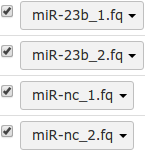
\includegraphics[scale=0.65]{figures/qc_01.png}\\
Hence, each pair of files belongs to each other and we can treat them as pairs in galaxy. First you have to select \textit{For all selected...} to apply actions on multiple history items at once, then you have to select those 2 history items you want to have as pair and then you have to select \textit{Build Dataset Pair}. Galaxy does not really know which one is the forward and which one is the reverse. Therefore make sure that \textbf{\_1 is forward} and \textbf{\_2 is reverse}. If galaxy choose the files correctly by it itself, use \text{Swap}. One of the samples has been treated with miR-23b and the other is a control. Make sure you use names that make this clear. After you have done this, you will see that you end up with 6 datasets in total, of which 2 pairs. To avoid confusion it is easier to hide the individual history items, leaving two items in the history:\\
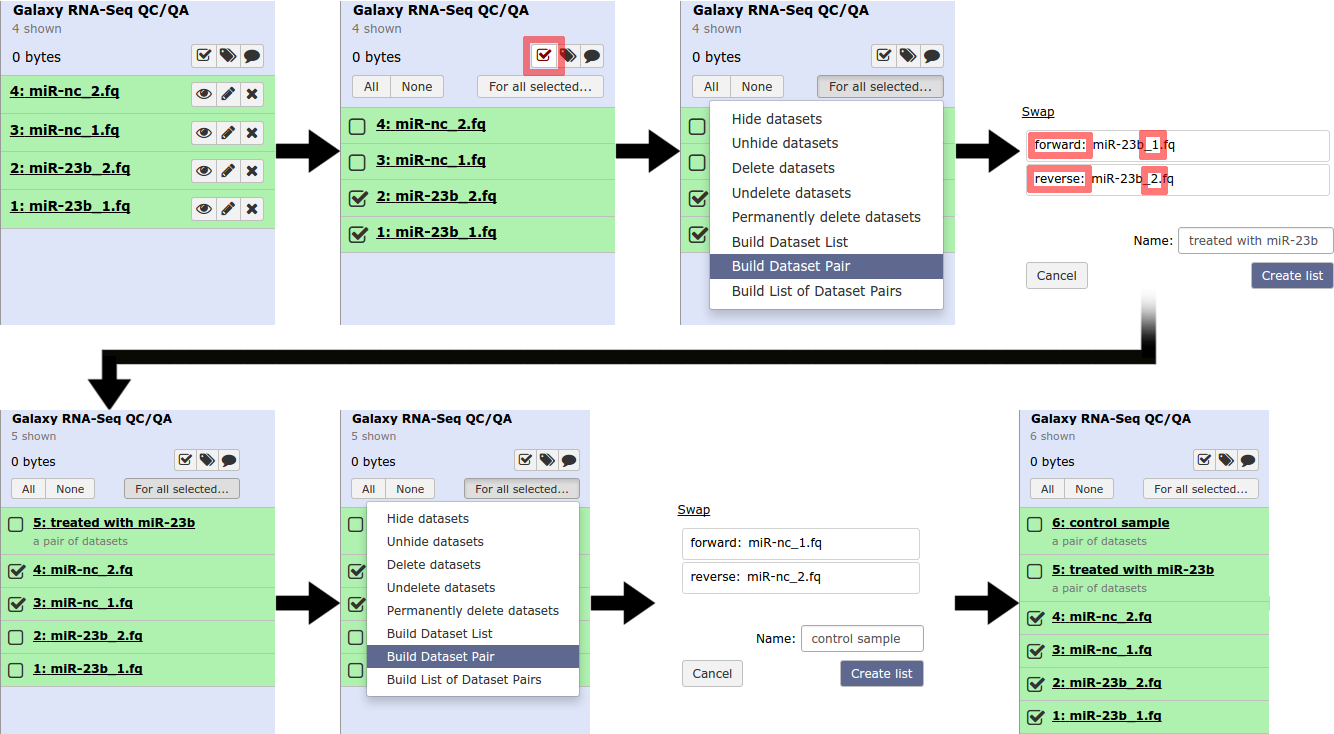
\includegraphics[width=\textwidth]{figures/qc_02.png}\\
\subsection{Fastq, Fastqsanger and FastQC}
To obtain statistics on the data, find the tool ``\textit{\underline{FastQC} Read Quality reports}''. This tool, originally developed for DNA-Seq analysis, makes several summaries of the data and presents the output in a HTML page. As you can see, by default FastQC selects the individual fastq files for analysis. This is because FastQC does analysis just on one fastq file. When we choose to select one of our pairs, galaxy will run FastQC twice and merge the results into a new pair:\\
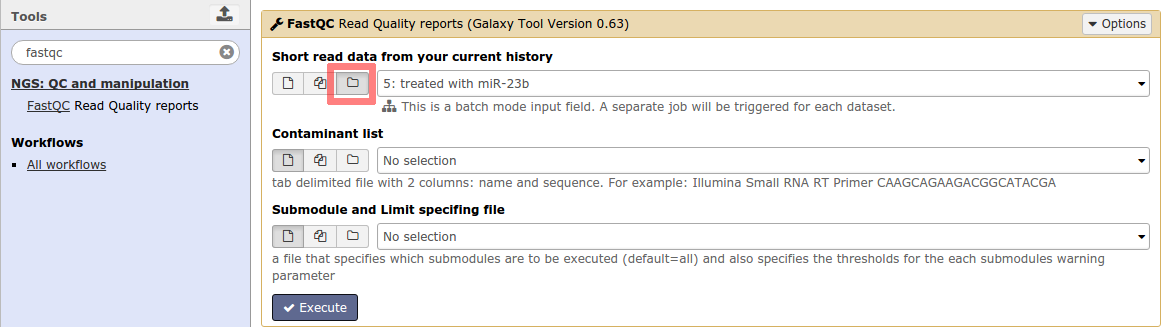
\includegraphics[width=\textwidth]{figures/qc_03.png}\\
What follows is a quality report (raw data and HTML report) for both the forward and the reverse pair. Go to \textit{Back to Galaxy RNA-Seq QC/QA FastQC on collection 5: Webpage \ldots} and open the report named \textit{forward} which should look similar to this:\\
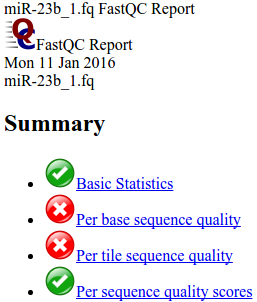
\includegraphics[scale=0.65]{figures/qc_04.png}\\
The galaxy history items are in the \textbf{fastq} format. This format is a general format that includes a few subformats based on different quality encodings. For the next step you need to understand the FASTQ encoding formats. They are described at the following website in section \textit{Encoding}:\\
\url{http://en.wikipedia.org/wiki/FASTQ\_format#Encoding}\\
In the FastQC report, scroll down to \textbf{Basic Statistics} and figure out what the \text{Encoding} is. This information may be important, especially because for certain older galaxy configurations, so write it down:\\
\verb|.......................................................|\\
The more or less standard encoding is \textit{fastqsanger}, which is the same encoding as \textit{Illumina 1.8} and \textit{Illumina 1.9}, also referred to as \textit{Illumina 1.8+}. To convert any fastq file to \textit{fastqsanger}, you can use the tool ``\textit{\underline{FASTQ Groomer} converts between various FASTQ quality formats}''. In here, make sure the quality encoding you wrote down matches the one in the input field. Further, make sure you run it twice; for each pair:\\
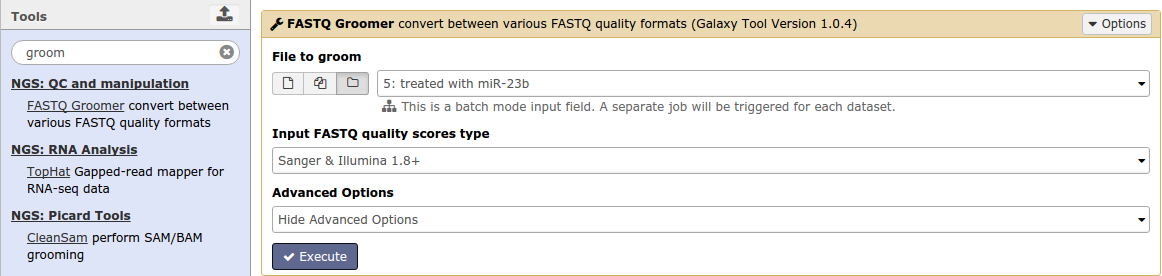
\includegraphics[width=\textwidth]{figures/qc_05.png}\\
This will add two new pairs to your history, with names that are not convenient. Please rename:
\begin{itemize}
	\item ``\textit{FASTQ Groomer on collection 5}'' to ``\textit{miR-23b (groomed)}''
	\item ``\textit{FASTQ Groomer on collection 6}'' to ``\textit{control sample (groomed)}''
\end{itemize}
If we go back to the FastQC webpage report, and look in section \textit{Per base sequence quality}, we see the average quality per base for all reads. The colors green, orange and red indicate whether the quality is considered good, okay, or bad. As you can see, the quality drops as the sequences get longer. It is important to realize that low quality bases will complicate alignment but also SNP detection, because there will be more mismatches. To improve the base quality of the data, we would like to:
\begin{itemize}
	\item Trim the low quality bases from the ends
	\item Remove reads of which the average quality is too low
	\item Remove reads that are too short
\end{itemize}
A tool that covers all of this is ``\textit{\underline{Sickle} windowed adaptive trimming of FASTQ data}''. For both pairs \textit{miR-23b (groomed)} and \textit{control sample (groomed)}, run it with the following settings:\\
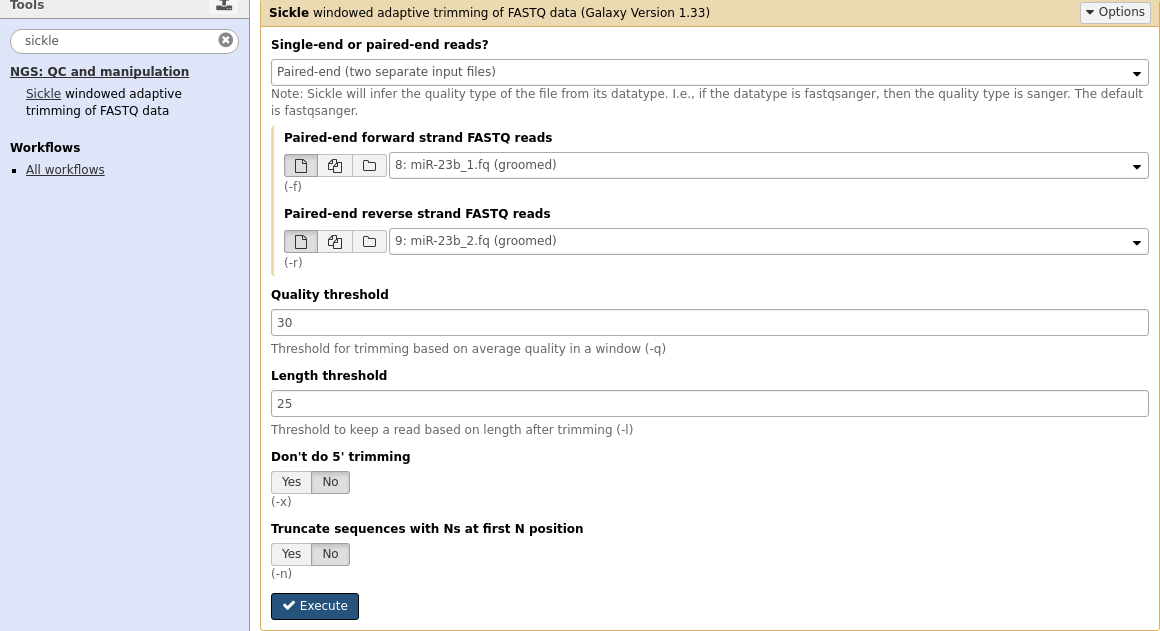
\includegraphics[width=\textwidth]{figures/qc_06.png}\\
Immediately after running a sickle analysis, rename the files 
\textit{Singletons from paired-end ...} and \textit{Paired-end output of Sickle on ...} to:
\begin{itemize}
	\item[] for miR-23b:
	\begin{itemize}
		\item miR-23b, singletons(clean)
		\item miR-23b (clean)
	\end{itemize}
	\item[] for control sample:
	\begin{itemize}
		\item control sample, singletons(clean)
		\item control sample (clean)
	\end{itemize}
\end{itemize}
If desired, you can hide the other results, such that you will get a history similar to:\\
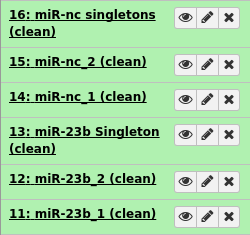
\includegraphics[scale=0.55]{figures/qc_07.png}\\
As you can see, Sickle produces for every set of paired sequencing reads, a set of pairs and an extra file with ``singletons''.
\begin{itemize}
	\item What would singletons be?
\end{itemize}
To confirm that the base quality has improved, run the FastQC again on \textit{ miR-23b (clean) }, and take a look at it:
\begin{itemize}
	\item Has the \textit{Per base sequence quality} improved?
	\item Have the per sequence quality scores improved?
	\item Why has the \textit{sequence length distribution} changed?
\end{itemize}
FastQC also has a section \textit{Overrepresented sequences}, indicated in red with a huge list. Apart from that we are using a truncated artificial dataset, it often happens in RNA-Seq data that these sequences appear. As said before, this tool was orignally written for DNA-Seq data.
\begin{itemize}
	\item Can you think of a biological reason why sequences could be overrepresented in RNA-Seq data?
\end{itemize}